\documentclass[tikz,border=2mm]{standalone}
\usepackage[T1]{fontenc}
\usepackage{lmodern}
\usetikzlibrary{arrows.meta, shapes.geometric, fit, backgrounds, calc}

\begin{document}
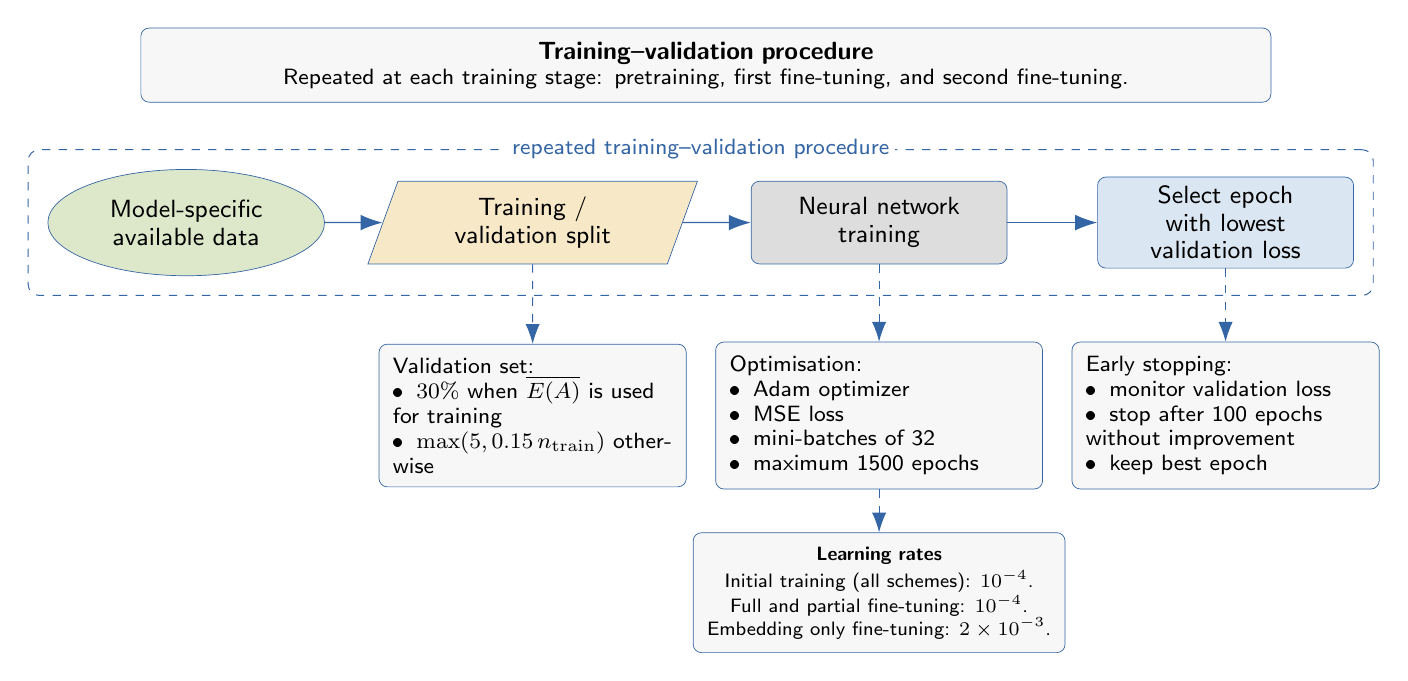
\begin{tikzpicture}[
  x=1cm,
  y=-1cm,
  font=\sffamily,
  >=Latex,
  blueLine/.style={draw=blueLine},
  block/.style={rounded corners=3pt, blueLine, fill=modelFill, line width=0.25pt,
                minimum width=3.25cm, minimum height=1.05cm,
                align=center, text width=2.85cm, font=\sffamily\fontsize{9}{10}\selectfont},
  data/.style={ellipse, blueLine, fill=dataFill, line width=0.25pt,
               minimum width=3.25cm, minimum height=1.10cm,
               align=center, text width=2.65cm, font=\sffamily\fontsize{9}{10}\selectfont},
  split/.style={trapezium, trapezium left angle=70, trapezium right angle=110,
                blueLine, fill=splitFill, line width=0.25pt,
                minimum width=3.25cm, minimum height=1.05cm,
                align=center, text width=2.65cm, font=\sffamily\fontsize{9}{10}\selectfont},
  eval/.style={rounded corners=3pt, blueLine, fill=evalFill, line width=0.25pt,
               minimum width=3.25cm, minimum height=1.05cm,
               align=center, text width=2.75cm, font=\sffamily\fontsize{9}{10}\selectfont},
  note/.style={rounded corners=3pt, blueLine, fill=noteFill, line width=0.25pt,
               align=left, text width=3.55cm, inner sep=5pt,
               font=\sffamily\fontsize{8}{9}\selectfont},
  stageNote/.style={rounded corners=3pt, blueLine, fill=noteFill, line width=0.25pt,
                    align=center, text width=14.0cm, inner sep=5pt,
                    font=\sffamily\fontsize{8}{9}\selectfont},
  phase/.style={rounded corners=4pt, blueLine, dashed, line width=0.35pt,
                inner sep=7pt},
  head/.style={font=\sffamily\fontsize{11}{13}\selectfont\bfseries, align=center},
  small/.style={font=\sffamily\fontsize{8}{9}\selectfont, align=center},
  arrow/.style={blueLine, line width=0.45pt, -{Latex[length=2.8mm,width=2mm]}},
  dashedarrow/.style={blueLine, line width=0.35pt, dashed, -{Latex[length=2.5mm,width=1.8mm]}}
]

\definecolor{blueLine}{RGB}{52,101,164}
\definecolor{dataFill}{RGB}{221,232,203}
\definecolor{splitFill}{RGB}{247,232,199}
\definecolor{modelFill}{RGB}{221,221,221}
\definecolor{evalFill}{RGB}{218,230,242}
\definecolor{noteFill}{RGB}{247,247,247}
\definecolor{redText}{RGB}{201,33,30}

\node[stageNote] (stages) at (6.6,0.30) {{\fontsize{9}{10}\selectfont\bfseries Training--validation procedure}\\Repeated at each training stage: pretraining, first fine-tuning, and second fine-tuning.};

% Main pipeline
\node[data, minimum width=2.75cm, minimum height=1.35cm, text width=2.25cm] (input) at (0,2.3) {\mbox{Model-specific}\\\mbox{available data}};
\node[split] (split) at (4.4,2.3) {Training / validation split};
\node[block] (train) at (8.8,2.3) {\mbox{Neural network}\\training};
\node[eval] (select) at (13.2,2.3) {Select epoch with lowest validation loss};

\draw[arrow] (input) -- (split);
\draw[arrow] (split) -- (train);
\draw[arrow] (train) -- (select);

% Make the scope of the repeated training procedure explicit.
\node[phase, fit=(input)(split)(train)(select)] (trainingphase) {};
\node[small, fill=white, inner sep=2pt, text=blueLine]
  at (trainingphase.north) {repeated training--validation procedure};

% Details below the pipeline
\node[note] (splitnote) at (4.4,4.75) {Validation set:\\
\textbullet\enspace $30\%$ when $\overline{E(A)}$ is used for training\\
\textbullet\enspace $\max(5, 0.15\,n_{\mathrm{train}})$ otherwise};
\draw[dashedarrow] (split.south) -- (splitnote.north);

\node[note, text width=3.8cm] (trainnote) at (8.8,4.75) {Optimisation:\\
\textbullet\enspace Adam optimizer\\
\textbullet\enspace MSE loss\\
\textbullet\enspace mini-batches of 32\\
\textbullet\enspace maximum 1500 epochs};
\draw[dashedarrow] (train.south) -- (trainnote.north);

\node[note] (earlynote) at (13.2,4.75) {Early stopping:\\
\textbullet\enspace monitor validation loss\\
\textbullet\enspace stop after 100 epochs without improvement\\
\textbullet\enspace keep best epoch};
\draw[dashedarrow] (select.south) -- (earlynote.north);

% Learning rates apply to the training stage, not to the validation split.
\node[note, text width={}, align=center,
      font=\sffamily\fontsize{7}{8}\selectfont] (rates) at (8.8,7.0) {
\textbf{Learning rates}\\[2pt]
Initial training (all schemes): $10^{-4}$.\\
Full and partial fine-tuning: $10^{-4}$.\\
Embedding only fine-tuning: $2\times10^{-3}$.
};
\draw[dashedarrow] (trainnote.south) -- (rates.north -| trainnote.south);

\end{tikzpicture}
\end{document}
